% Default course lecture note template by asp 
\documentclass[letterpaper]{article}
\usepackage[utf8]{inputenc}
\usepackage[T1]{fontenc}
\usepackage[english]{babel}
\usepackage[top=3cm, bottom=3cm, left=3.85cm, right=3.85cm]{geometry}
\usepackage[onehalfspacing]{setspace}
\usepackage{amsmath,amsthm,amssymb,wasysym,fdsymbol,marvosym}
\usepackage{graphicx}
\usepackage[usenames,dvipsnames]{color}

\newtheoremstyle{xxx}
  {0pt}{1pt}
  {\color{BrickRed}}
  {0pt}
  {\bf}{.}{ }{}
\newtheoremstyle{yyy}
  {0pt}{1pt}
  {\color{OliveGreen}}
  {0pt}
  {\bf}{.}{ }{}
\newtheoremstyle{zzz}
  {0pt}{1pt}
  {\color{Blue}}
  {0pt}
  {\bf}{.}{ }{}
\newtheoremstyle{evil}
  {2pt}{2pt}
  {\color{red} \bf}
  {0pt}
  {\bf}{.}{ }{}

\theoremstyle{xxx}
\newtheorem{thrm}{Theorem}
\newtheorem{thrm-s}{Sanity Check}
\newtheorem{prop}{Proposition}
\theoremstyle{evil}
\newtheorem{warn}{Warning}
\newtheorem{evil}{Evil}
\theoremstyle{yyy}
\newtheorem{corl}{Corollary}
\newtheorem{lmma}{Lemma}
\theoremstyle{plain}
\newtheorem{expl}{Example}
\theoremstyle{zzz}
\newtheorem{defn}{Definition}

\newcommand{\notn}{\paragraph{Notation.}}
\newcommand{\recl}{\paragraph{Recall.}}
\newcommand{\rmrk}{\paragraph{Remark.}}
\newcommand{\note}{\paragraph{Note.}}

\newcommand{\ftwo}{\mathbb{F}_2}
\newcommand{\fttwo}{\mathbb{F}_{32}}
\newcommand{\binrep}[1]{\left\{#1\right\}}

\begin{document}

% Two-column title block
\begin{minipage}[b]{0.7\linewidth}
{\huge The Math Behind the Volvelles}
\end{minipage}
\begin{minipage}[b]{0.3\linewidth}
  \begin{flushright}
    Andrew Poelstra\\
    2021 November 27
  \end{flushright}
\end{minipage}
\\

% Actual content start
\section{Mathematical Preliminaries}

In this first section we give a crash course in field theory. Readers familiar
with this material should have no problem skipping or skimming this section,
at least up to Section \ref{sec:sss}.
Readers who are completely unfamiliar with this material are unlikely to be
able to follow the condensed exposition, and are encouraged to consult
standard algebra textbooks (e.g. the one by Dummit and Foote) or Wikipedia.

\subsection{Fields and $\ftwo$}
Consider the integers modulo 2. This is a set consisting of two equivalence
classes, the evens and the odds, which hereafter we will refer to as 0 and 1.
This set is a \textbf{field}, which means that when we define addition and
multiplication in the obvious way, it satisfies the following axioms:
\begin{enumerate}
\item The set is closed under addition; addition is associative, commutative,
has an identity element 0, and all elements have additive inverses. In other
words it is an \textbf{abelian group} under addition.
\item Similarly it is an abelian group under multiplication, with identity 1.
\item The \textbf{distributive law} holds, which means that $a(b + c)$ always
equals $ab + ac$.
\end{enumerate}

We refer to this field as $\ftwo$. For any field, we refer to its nonzero
elements as the \textbf{multiplicative group} of the field. We observe that
the multiplicative group of $\ftwo$ has only the identity element.

\subsection{Polynomial Rings}

Since $\ftwo$ has only two elements, it is hard to do interesting algebra on
it. But it is a fact that, by adjoining a formal symbol $x$ to a field, we
can obtain a much bigger (in fact, countably infinite) set of \emph{polynomials}
in $\ftwo$. We denote this set $\ftwo[x]$ and call it the \textbf{polynomial
ring} of the field.

Formally, the set of polynomials is defined as

\[ \left\{ \sum_{i=0}^n a_ix^i : n\in\mathbb{N}\cup\{0\}, a_i\in \ftwo  \right\} \]

A ring, for our purposes, is defined the same way as a field except that we do
not require multiplication to be invertible. It is easy to check that the
polynomial ring, endowed with addition and multiplication in the obvious ways,
is in fact a ring.

For a polynomial of the form $\sum_{i=0}^n a_ix^i$ we refer to $n$ as the
\textbf{degree} of the polynomial. It is an elementary fact that the product
of polynomials has degree equal to the sum of the degrees of the factors.

We refer to polynomials of degree 0 is \textbf{constant polynomials}. It is
also a fact that a polynomial has a multiplicative inverse, i.e. it is a
\textbf{unit}, if and only if it is constant.

If a polynomial $r$ can be written as the product of two polynomials as $r=pq$,
where neither $p$ nor $q$ are units (degree 0) we say that $r$ is
\textbf{irreducible}.

\subsection{Quotient Fields}

Just like we can consider the integers modulo some integer $n$, thus obtaining
$n$ equivalence classes which inherit (roughly) the original ring structure of
the integers, we can consider a polynomial ring modulo some polynomial $p$. In
this case, we will get $m^n$ equivalence classes, where $m$ is the number of
elements in the underlying field and $n$ is the degree of the polynomial. For
our purposes $m$ is always 2, so we get $2^n$ elements.

We call the set of equivalence classes a \textbf{quotient ring}, and its addition
and multiplication are defined in the obvious way.

Just like in the integer case, if our polynomial $p$ can be factored into
nonconstant polynomials as $p=p_1p_2$, their images in the quotient ring will
be nonzero but satisfy $p_1p_2 = 0$. In other words they are \textbf{zero
divisors} and imply that multiplication in the ring is not invertible.

We do not like zero divisors, so from here on out we will be sure to mod out
our polynomial ring only by irreducible polynomials. It is a fact that the
resulting quotient ring will then be a field, and we term in a \textbf{quotient
field}. It is a fact that $x^5 + x^3 + 1$ is irreducible in $\ftwo$, so that
$\ftwo/(x^5 + x^3 + 1)$ is a quotient field with 32 elements.

In this field the object $x$ is a field element with a distinct identity and
algebraic properties, so we rename it $\alpha$ to preserve the symbol $x$ to
be an indeterminate used for writing polynomials.

It is a fact that, for this specific polynomial, that $\alpha$ is a
\textbf{generator} of the quotient field, meaning that the field in its entirety
is equal to
\[ \left\{ \alpha^i : i \in \{0,1,\ldots,30\} \right\} \]
and zero.

We observe that the order of the multiplicative group is 31, a prime, and therefore
every element of the group except 1 is a generator of the group. Furthermore there
are no nontrivial proper subgroups. These are an elementary facts of group theory.

We refer to this new field as $\fttwo$. It is fact of field theory that all
groups with 32 elements are isomorphic to this one, which justifies the name.
But bear in mind that, for our purposes, the group was constructed as $\ftwo[x]/
(x^5 + x^3 + 1)$ and has a distinguished generator $\alpha$ which is a root
of that polynomial.

\subsection{Vector Spaces}

We observe that $\fttwo$ is a \textbf{vector space} over $\ftwo$. A vector
space $V$ over a field $\mathbb{F}$ is defined by the following axioms:

\begin{enumerate}
\item $V$ is an abelian group with operation $+$ and identity $0_V$.
\item $(a + b)v = av + bv$ and $a(u + v) = au + av$ for all $a,b\in \mathbb{F}$ and
$u,v\in V$.
\end{enumerate}

We refer to a finite sum of the form $\sum_i f_iv_i$ with $f_i\in \mathbb{F}$ and
$v_i\in V$ as a \textbf{linear combination}. We observe that every element
of $\fttwo$ is a linear combination of the elements $\{1,\alpha,\alpha^2,
\alpha^3,\alpha^4\}$, and that no smaller set of elements has this property.
We call such a set a \textbf{basis} for $\fttwo$.

\subsection{Lagrange Interpolation and Shamir's Secret Sharing\label{sec:sss}}

Let $\mathbb{F}$ be a field and $p$ a polynomial of degree $n$ in $\mathbb{F}[x]$. It is a
standard theorem of algebra that $p$'s value on all points of $\mathbb{F}$ is
implied by its values on any $n+1$ distinct points.

As discovered by Edward Waring in 1779, and later by Joseph-Louis Lagrange
in 1795\footnote{citation: Wikipedia}, it is actually possible to compute
the value of a polynomial at a field element $x$ explicitly in terms of
its values at $n$ given distinct points $x_i$.

Specifically, suppose that $p(x_i) = y_i$. Then
\begin{equation}
 p(x) = \sum_{i=1}^{n+1} y_i \ell_i(x) \label{eq:linterp}
\end{equation}
where $\ell_i$ is determined entirely by the $x_i$'s, as
\[ \ell_i(x) = \prod_{j\neq i} \frac{x - x_j}{x_i - x_j} \]

There are several very interesting observations to be made here:
\begin{enumerate}
\item First, for a fixed set of $x_i$'s, we see that the vector space of
$n$-degree polynomials over $\mathbb{F}$ is spanned by the set $\{\ell_i(x)\}$. Since
there are $n+1$ polynomials and this space has dimension $n+1$ (an obvious
basis for it is $\{ 1,x,x^2,\ldots,x^n\}$), this means that the set
$\{\ell_i(x)\}_i$ forms a basis for this space.
\item Further, these basis polynomials satisfy the equality
$\sum_i \ell_i(x) = 1$. (One way to see this is by using equation
\eqref{eq:linterp} to interpolate the constant one polynomial.)

This means that equation \eqref{eq:linterp} is an \textbf{affine
combination} of the $y_i$'s, a strengthening of the familiar notion
of linear combination. This property will become important, as we
will see.
\item If we further fix $x$, we see that knowing $p$'s evaluation at
every $x_i$ is sufficient to determine $p(x)$, while knowing any fewer
evaluations provides zero information about $x$: suppose for example
that $y_n$ is unknown. Then by a suitable choice of $y_n$ in \eqref{eq:linterp}
we can cause $p(x)$ to take any of the $|\mathbb{F}|$ possible values.
\end{enumerate}

Putting these facts together, we obtain \textbf{Shamir's Secret Sharing
Scheme} (SSSS) for splitting a secret element of $\mathbb{F}$ into up to $|\mathbb{F}|-1$
shares, such that a fixed threshold number $k$ of them are sufficient
to reconstruct the secret:

\begin{enumerate}
\item First, fix an index $s\in \mathbb{F}$ to be the secret index.
\item Generate a random $(k-1)$-degree polynomial $p$ by choosing $k$
random values and assigning them to be the evaluation of $p$ at specific
points $x_i\in \mathbb{F}$.

(If the secret is known beforehand, then fix $p(s)$ to be the secret
and generate $k-1$ other evaluations of $p$. randomly.)
\item Distribute the points $x_i$ along with their evaluations $p(x_i)$
to multiple parties.
\item Then if any $k$ of them come together, they can use equation
\eqref{eq:linterp} to reconstruct the secret $p(s)$.
\end{enumerate}

We call the $k$ randomly generated values \textbf{initial shares} and
every other evaluation of $p$ a \textbf{derived share}.

There are several interesting observations here:
\begin{itemize}
\item If we have a sequence $F_x = \{f_i\}$ of elements of $\mathbb{F}$, we can use
SSSS in parallel on all of them, choosing independently random polynomials
$\{p_i\}$ and distributing the sequence $\{p_i(x)\}$ along with the evaluation
point $x$.
\item If, for some particular $i$, $f_i$ is constant across our $k$ initial
shares $F_{x_1},\ldots,F_{x_k}$, Lagrange interpolation will cause the same
constant to appear in the same position for all derived shares. So you can
have, say, a fixed header on all of your shares which will be preserved by
the secret-sharing mechanism.
\item Similarly, for some particular $i$, you set $f_i=x$, i.e. you encode the
evaluation point in a fixed place in your sequence, then Lagrange interpolation
will interpolate the polynomial $p(x) = x$ here and place the correct value
of $x$ in the correct place for all shares.
\item Going even further, suppose for each initial share $F_x=\{f_i\}$, some fixed
affine relation holds among the $f_i$'s, e.g.
\[ \sum_i \alpha_i f_i = \beta \]
for fixed $\beta,\alpha_i\in \mathbb{F}$. Then this fixed affine relation
\emph{will continue to hold for all derived shares}!

This is not immediately obvious but can be shown by direct computation and
using the fact that Lagrange interpolation is an affine combination of $f_i$'s.
\end{itemize}

This fact is so important that we term it the \textbf{Fundamental Theorem of
Computing SSSS with Volvelles}. The Fundamental Theorem implies that if we
apply any checksum derived from a linear code (or a linear code plus a
constant) to our initial shares, that the derived shares will automatically
be checksummed as well.

For more information about volvelles, see the next two sections.

\subsection{The Bech32 Alphabet}

The previous section indicated that if $\beta\in\fttwo$, then we can write
\[ \beta = b_4\alpha^4 + b_3\alpha^3 + b_2\alpha^2 + b_1\alpha + b_0 \]
where each $b_i\in\{0, 1\}$. We can therefore encode $\beta$ as a 5-bit
number by directly encoding the bits $b_i$. Alternately, since there are
only 32 such $\beta$s, we assign them all alphanumeric symbols, with four
symbols to spare. This is the premise behind the \textbf{bech32 alphabet},
defined in BIP 173, and reproduced on the following page.

In addition to the bech32 alphabet, which uses Latin characters, we also use
an alternate alphabet using Greek letters and various symbols.

We have ordered all the symbols in three ways -- $\alpha$betically,
alphabetically, and by their ``numeric'' binary value. These three
representations are useful in different contexts:
\begin{enumerate}
\item Representing elements as a power of $\alpha$ makes multiplication
very easy, since multiplication is just addition mod 32 in the exponent.

This is how our multiplication wheel can be implemented as a slide ruler.
\item Representing alphabetically makes it easy for humans to scan and sort.
\item Representing in binary is how the elements are typically stored in
computers, can be used to convert data from other encodings. Addition is
simply xor in this format.
\end{enumerate}

\clearpage
~\\~\\~\\~\\ % vertical centering

% Ordered by power
\begin{minipage}[b]{0.3\linewidth}
\begin{center}
\begin{tabular}{|cccc|}
\hline
Q & $\times$   & - & 00000 \\
P & $\aleph$   & $\alpha^0$ & 00001 \\
Z & $\alpha$   & $\alpha^1$ & 00010 \\
Y & $\Gamma$   & $\alpha^2$ & 00100 \\
G & $\Theta$   & $\alpha^3$ & 01000 \\
S & $\Psi$     & $\alpha^4$ & 10000 \\
F & $\Lambda$  & $\alpha^5$ & 01001 \\
J & @          & $\alpha^6$ & 10010 \\
D & $\rho$     & $\alpha^7$ & 01101 \\
6 & \textdagger& $\alpha^8$ & 11010 \\
A & $\P$       & $\alpha^9$ & 11101 \\
N & \#         & $\alpha^{10}$ & 10011 \\
0 & $\Phi$     & $\alpha^{11}$ & 01111 \\
7 & $\blacklozenge$ & $\alpha^{12}$ & 11110 \\
4 & $\cent$    & $\alpha^{13}$ & 10101 \\
R & $\beta$    & $\alpha^{14}$ & 00011 \\
X & $\epsilon$ & $\alpha^{15}$ & 00110 \\
V & $\Pi$      & $\alpha^{16}$ & 01100 \\
C & \textcurrency & $\alpha^{17}$ & 11000 \\
E & $\oplus$   & $\alpha^{18}$ & 11001 \\
M & \textdaggerdbl & $\alpha^{19}$ & 11011 \\
L & $\varheartsuit$ & $\alpha^{20}$ & 11111 \\
H & \EUR       & $\alpha^{21}$ & 10111 \\
8 & $\eta$     & $\alpha^{22}$ & 00111 \\
W & $\Sigma$   & $\alpha^{23}$ & 01110 \\
U & $\S$       & $\alpha^{24}$ & 11100 \\
3 & $\Omega$   & $\alpha^{25}$ & 10001 \\
T & $\Xi$      & $\alpha^{26}$ & 01011 \\
K & \yen       & $\alpha^{27}$ & 10110 \\
9 & $\Delta$   & $\alpha^{28}$ & 00101 \\
2 & $\mu$      & $\alpha^{29}$ & 01010 \\
5 & \%         & $\alpha^{30}$ & 10100 \\
\hline
\end{tabular}
\end{center}
\end{minipage}
% Ordered by alphabet
\begin{minipage}[b]{0.3\linewidth}
\begin{center}
\begin{tabular}{|ccc|}
\hline
A & $\alpha^9$ & 11101 \\
C & $\alpha^{17}$ & 11000 \\
D & $\alpha^7$ & 01101 \\
E & $\alpha^{18}$ & 11001 \\
F & $\alpha^5$ & 01001 \\
G & $\alpha^3$ & 01000 \\
H & $\alpha^{21}$ & 10111 \\
J & $\alpha^6$ & 10010 \\
K & $\alpha^{27}$ & 10110 \\
L & $\alpha^{20}$ & 11111 \\
M & $\alpha^{19}$ & 11011 \\
N & $\alpha^{10}$ & 10011 \\
P & $\alpha^0$ & 00001 \\
Q & - & 00000 \\
R & $\alpha^{14}$ & 00011 \\
S & $\alpha^4$ & 10000 \\
T & $\alpha^{26}$ & 01011 \\
U & $\alpha^{24}$ & 11100 \\
V & $\alpha^{16}$ & 01100 \\
W & $\alpha^{23}$ & 01110 \\
X & $\alpha^{15}$ & 00110 \\
Y & $\alpha^2$ & 00100 \\
Z & $\alpha^1$ & 00010 \\
0 & $\alpha^{11}$ & 01111 \\
2 & $\alpha^{29}$ & 01010 \\
3 & $\alpha^{25}$ & 10001 \\
4 & $\alpha^{13}$ & 10101 \\
5 & $\alpha^{30}$ & 10100 \\
6 & $\alpha^8$ & 11010 \\
7 & $\alpha^{12}$ & 11110 \\
8 & $\alpha^{22}$ & 00111 \\
9 & $\alpha^{28}$ & 00101 \\
\hline
\end{tabular}
\end{center}
\end{minipage}
% Ordered by binary
\begin{minipage}[b]{0.3\linewidth}
\begin{center}
\begin{tabular}{|ccc|}
\hline
Q & - & 00000 \\
P & $\alpha^0$ & 00001 \\
Z & $\alpha^1$ & 00010 \\
R & $\alpha^{14}$ & 00011 \\
Y & $\alpha^2$ & 00100 \\
9 & $\alpha^{28}$ & 00101 \\
X & $\alpha^{15}$ & 00110 \\
8 & $\alpha^{22}$ & 00111 \\
G & $\alpha^3$ & 01000 \\
F & $\alpha^5$ & 01001 \\
2 & $\alpha^{29}$ & 01010 \\
T & $\alpha^{26}$ & 01011 \\
V & $\alpha^{16}$ & 01100 \\
D & $\alpha^7$ & 01101 \\
W & $\alpha^{23}$ & 01110 \\
0 & $\alpha^{11}$ & 01111 \\
S & $\alpha^4$ & 10000 \\
3 & $\alpha^{25}$ & 10001 \\
J & $\alpha^6$ & 10010 \\
N & $\alpha^{10}$ & 10011 \\
5 & $\alpha^{30}$ & 10100 \\
4 & $\alpha^{13}$ & 10101 \\
K & $\alpha^{27}$ & 10110 \\
H & $\alpha^{21}$ & 10111 \\
C & $\alpha^{17}$ & 11000 \\
E & $\alpha^{18}$ & 11001 \\
6 & $\alpha^8$ & 11010 \\
M & $\alpha^{19}$ & 11011 \\
U & $\alpha^{24}$ & 11100 \\
A & $\alpha^9$ & 11101 \\
7 & $\alpha^{12}$ & 11110 \\
L & $\alpha^{20}$ & 11111 \\
\hline
\end{tabular}
\end{center}
\end{minipage}

\clearpage

\subsection{Volvelles}

Volvelles, or slide charts, are computers constructed by two sheets of paper, cut
into circles and affixed at the center so that they are able to rotate relative
to each other.

\begin{center} 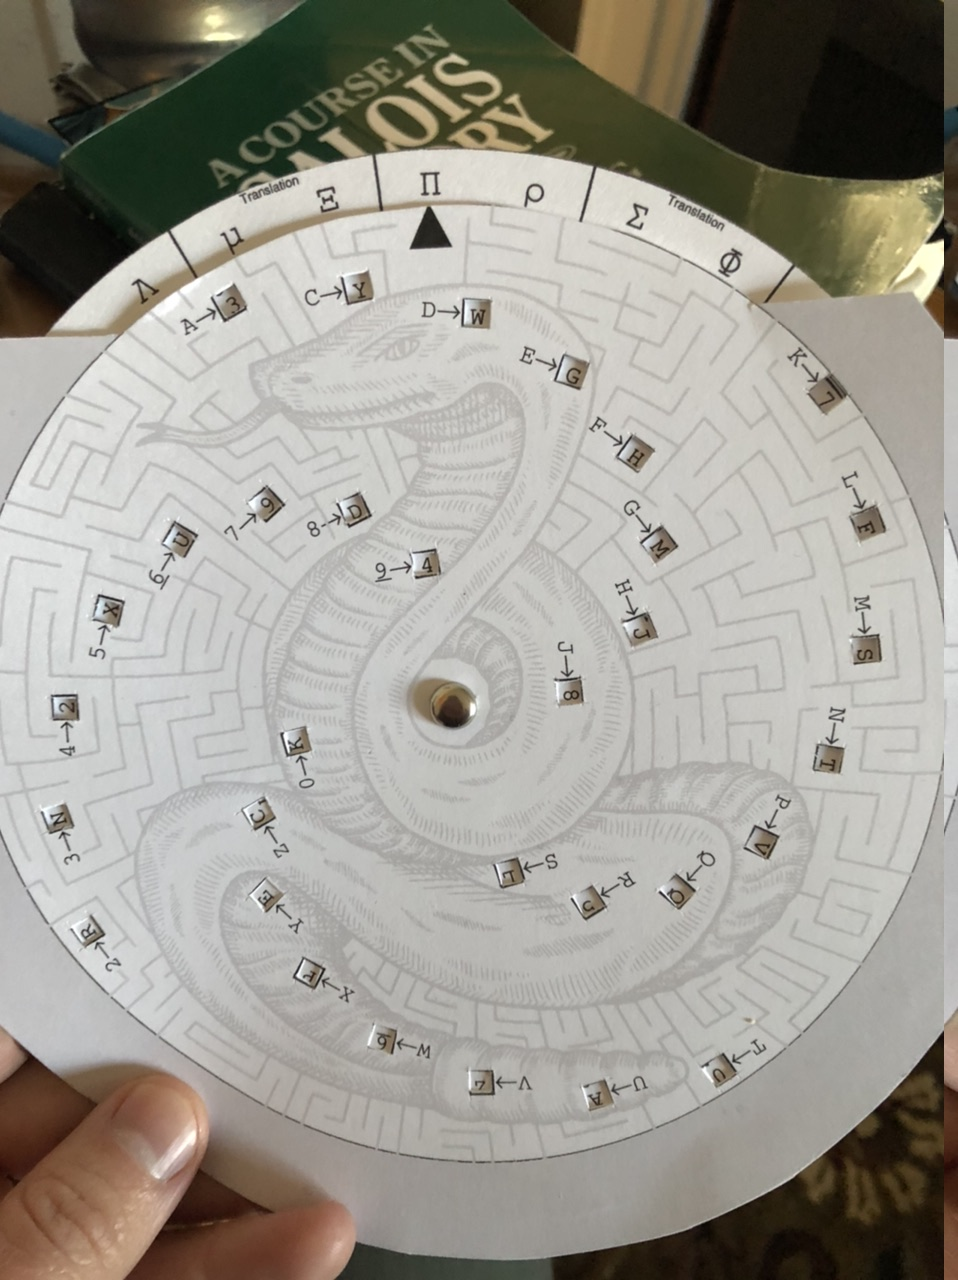
\includegraphics[scale=0.35]{volvelle.jpeg} \end{center}

The top sheet has holes cut into it, selectively revealing data printed on the
bottom sheet, depending on the rotation. The top sheet has a pointer used to
index the data being revealed.

\paragraph{Volvelles and Algebraic Structure.} Our volvelles have 32 holes cut
in the face, corresponding to the 32 bech32 characters. If all 32 positions
of the volvelle revealed distinct locations on the bottom wheel, it would
require symbols to be printed on the bottom wheel in 1024 positions. If there
were algebraic structure relating the results of different volvelle positions,
we could reduce this number.

As an extreme example, consider the case of multiplication. In this case, we
exclude $0\in\fttwo$ and have only 31 positions and 31 values to reveal. By
ordering the positions of the wheel as increasing powers of $\alpha$, and the
entries on the front of the wheel as decreasing powers of $\alpha$, then every
turn of the volvelle would simply all the revealed symbols by one window, and
there would not ever even be unrevealed symbols. In this case we can simplify
the design to a \textbf{circular slide ruler}.

%% TODO put pic here

In the case of the other volvelles, we are not so lucky, and we have been forced
to print all 1024 symbols on the bottom wheel, necessitating small (though usable)
windows and more importantly, leaving us with the uncomfortable feeling that we
are leaving algebraic structure unexploited. It is an open question whether we can
improve this, but let me argue here that we cannot.

Consider the case of the addition (xor) volvelle. One natural idea to consider
is that the value in the top window (labelled $A\rightarrow$) must always differ
from the value in the bottom window (labeled $T\rightarrow$) by $K=A-T$. So
if we were put the $A$ and $T$ windows at the same radius from the center, rotated
180 degrees from each other, we could use the same set of 32 bottom symbols for
both windows, reducing the density by two.

Unfortunately, this reduction depends on the fact that the $A$ \emph{index} and
$T$ \emph{index} are also rotated 180 degrees from each other. But then one rotation
later, the $C$ and $U$ indices are 180 degrees from each other, and these have a
different sum than $A$ and $T$.

In general, to accomplish this, we would need to mod our group out by $K$ additively
and then take all the two-element cosets and place their entries on opposite sides
of the addition wheel. The result, no matter what element you mod out by and no matter
how you order the cosets, is unnatural and confusing to use\footnote{I did not try
all possibilities exhaustively, so I could be wrong here. But I really doubt it.}.
From a user point of view, it is necessary that all the volvelle indices be in
alphabetical order, or very nearly so, or else the volvelle is slow and confusing
to use.

Similar considerations apply to the other two volvelles.

\paragraph{Which Volvelles Are There?} We have all the preliminary tools under
our belt to list the 3 volvelles and slide ruler, and what they do:

\begin{itemize}
\item The \textbf{Addition Volvelle} computes addition between bech32 characters.
As observed above, this corresponds to the xor function on their binary representation.
\item The \textbf{Translation Volvelle} computes multiplication between a symbol
character and a bech32 character. 
\item The \textbf{Recovery Volvelle}, turned to bech32 character $x$, and viewing
window $y$, computes the symbolic character corresponding to $(y + S)/(x + y)$.
\item The \textbf{Multiplication Wheel} is a circular slide ruler which performs
multiplication between two symbol characters.
\end{itemize}

We see now the justification for having two alphabets: both share creation and
and secret recovery are implemented as Lagrange interpolation using Equation
\eqref{eq:linterp} on page \pageref{eq:linterp}. In that equation, we are performing
a linear combination of $y_i$ values, which are secret shares encoded as bech32
characters. These values are exclusively multiplied by Lagrange basis polynomials,
which are always products of terms of the form $(x + y)/(x + z)$.

The process then, to do Lagrange interpolation, is to determine the $\ell_i(x)$
polynomial evaluated at the target share $x$ (the share to create, or $S$ in the case
of recovery), which can be done either using lookup tables or by finding component
symbols on the Recovery Volvelle and multiplying them together using the Multiplication
Wheel. Next, multiply each share $y_i$ by the resulting $\ell_i(x)$, using the Translation
Volvelle, and add them together using the Addition Volvelle.

In short, the bech32 alphabet is used for share values and share indices (which must
use the same alphabet since the index is encoded in the share itself) while the
symbol alphabet is used for Lagrange basis polynomials and their factors. The user
never needs to add basis polynomials and never needs to multiply share values, so
providing this capability would serve only to enable wrong turns.

Unfortunately, it is still possible (and not difficult) for the user to confuse
share values and share indices. I don't believe there is any way to avoid this.

\subsection{BCH Codes}

The final preliminary we need is that of a \textbf{BCH code}. There is a
rich and enormous theory underlying BCH codes, and linear codes in general,
but we will take an operationalist point of view:

An \textbf{error-correcting code} is a mapping from a set of raw data, called
\textbf{messages} into a larger set of \textbf{codewords} which have
some extra algebraic structure. In particular, between every pair of
codewords there is a minimum \textbf{distance}, which measures the
number of characters at which the two codewords differ.

Since all codewords differ by at least the minimum distance $d$, if there
are at most $d-1$ errors in a codeword, the result is guaranteed not to
be a valid codeword, and to be detected as a codeword. If there are fewer
than $d/2$ errors, the correct codeword is uniquely determined by being
the closest codeword to the actual received text, which means that this
number of errors can actually be corrected.

A \textbf{BCH code} is a specific type of error-correcting code. In a BCH
code, codewords are constructed by encoding data as the coefficients of a
large polynomial, then affixing some number of \textbf{checksum characters}.
The checksum characters are chosen such that the resulting polynomial is in
a specific residue class modulo a \textbf{generator polynomial} $G$.

Given a potential codeword, there is a unique minimum-degree polynomial
equivalent to this codeword modulo $G$, which can be found by modular
reduction. We refer to this reduced polynomial as the \textbf{reside}
of the codeword.

There are several properties of a BCH code that we will need:
\begin{itemize}
\item The \textbf{degree} of the code is the degree the roots of its
generator polynomial. (Since the polynomial is not, in general, irreducible,
this is \emph{not} the degree of the generator polynomial.)

The degree of our BCH code, and that of bech32, is 2. Degree-1 BCH codes are
called \textbf{Reed-Solomon codes}.
\item The $m$-value is the specific residue that all codewords must 
must have. All $m$ values are equivalent, in the sense that it is easy
to convert from one $m$ value to another (simply add the difference to
the checksum characters, modulo $G$).

But $m=0$ has the particularly bad property that any codeword can be extended
by addition of an arbitrary number of 0s to get another valid codeword. (This
highlights the fact that BCH codes are designed to handle only \emph{substitution}
or \emph{erasure} errors, not insertions or deletions.) Other small values of
$m$ have similar issues; bech32 was originally defined to have $m=1$ but later
needed to be modified to bech32m for this reason. bech32m uses a large random
$m$ instead.

On the other hand, $m=0$ makes a BCH code a \textbf{linear code}, and brings
with it a ton of algebraic properties which are needed for analysis, so this
is what is used in the literature.

In practice it is common to use a string of all-bits-one for $m$. For our code,
we chose characters which spell out \texttt{SECRETSHARE32}.

\item The \textbf{checksum length} is the number of extra characters that
need to be added to a string to ensure that it has the correct residue.
This value \emph{is} the degree of the generator polynomial.
\end{itemize}

We will return to BCH codes in the main text, when we discuss the Checksum
Worksheet and the properties of BCH codes which make them compatible with
Shamir's Secret Sharing.

\section{The Checksum}

We now get into the meat of the document, where we descibe how the actual
user processes are implemented. We start with the checksum.

\subsection{The Math}
Our checksum is defined by a BCH code with generator polynomial
\begin{align*}
    G(x) = x^{13}
        &+ \binrep{31}x^{12} + \binrep{5}x^{11} + \binrep{3}x^{10} + \binrep{28}x^9 + \binrep{0}x^8 + \binrep{31}x^7\\
        &+ \binrep{31}x^6 + \binrep{31}x^5 + \binrep{9}x^4 + \binrep{5}x^3 + \binrep{30}x^2 + \binrep{2}x + \binrep{2}
\end{align*}

Here the notation $\binrep{n}$ means that the binary expansion of $n$ should be
interpreted as the binary encoding of a $\fttwo$ element. That is, with $\alpha$
the standard generator of $\fttwo$,
\[ \binrep{\sum_i 2^ib_i} \mapsto \sum_i \alpha^ib_i \]

To checksum a string of bech32 characters $\{v_i\}_{i=1}^n$, we want to encode it
as a polynomial
\[ p(x) = x^n + \sum_{i=0}^{n-1} v^{n-i} x^n \]
such that $p(x)$ mod $G(x)$ is equal to \texttt{SECRETSHARE32}, or
\begin{align*}
r(x) =
    &\binrep{16}x^{12} + \binrep{25}x^{11} + \binrep{24}x^{10} + \binrep{3}x^9 + \binrep{25}x^8 + \binrep{11}x^7\\
    &+ \binrep{16}x^6 + \binrep{23}x^5 + \binrep{29}x^4 + \binrep{3}x^3 + \binrep{25}x^2 + \binrep{17}x + \binrep{10}
\end{align*}
Remembering throughout that an $n$-degree polynomial has $(n+1)$ terms, the way that
we do this is to concatenate the target residue \texttt{SECRETSHARE32} to our message
$\{ v_i \}$, compute the resulting residue
\begin{equation}
 \hat{p}(x) = x^{n+13} + \sum_{i=0}^{n+13-1} v^{n+13-i} x^{i} \textnormal{ mod } G(x)
 \label{eq:modg}
\end{equation}
We call the thirteen resulting characters the \texttt{checksum} and replace our
copy of \texttt{SECRETSHARE32} with them

Why does this work? Our goal is to find a checksum such that, when it is concatenated
to our original message, we get the correct residue mod $G(x)$. In Equation \eqref{eq:modg},
we multiplied our original message by $x^{13}$ (whose residue would then be the negation
of our checksum, minus the target residue) and added our target residue, to get the
negation of our checksum. Remember that in $\fttwo$ negation is a no-op, so we're done.

\subsection{The Worksheet}

\section{Secret Sharing}


\end{document}

